\section{R-Bäume}
R-Bäume funktionieren ähnlich wie B*-Bäume, erlauben jedoch mehrdimensionale Indizes.
Die maximale Kapazität eines Knotens (sowohl Blatt als auch innerer) wird dabei mit $M$ bezeichnet.
Die minimale Auslastung eines Knotens beträgt $m$, das wir für diese Übung als $m = \lfloor\frac{M}{2}\rfloor$ wählen.

\begin{note}
	Nicht aus der Vorlesung bekannt.
\end{note}

\begin{solution}
	Zunächst ein paar allgemeine Anmerkungen zu Vorgehen und Algorithmen.

	Der B*-Baum ist der eindimensionale Spezialfall eines R-Baums.

	Der wichtigste Algorithmus ist das Auffinden von Einträgen.
	Dazu geht man folgendermaßen vor:
	\begin{enumerate}
		\item Als Eingabe für den Suchalgorithmus dient ein Rechteck R.
		Gesucht werden alle Einträge, die R schneiden.
		(Alternativ könnte auch spezifiziert werden, dass nur Einträge gesucht werden, die komplett in R liegen o.\,ä.)
		\item Sei L die Wurzel.
		\item Falls L ein Blatt ist, gebe alle Einträge aus L zurück, die R schneiden.
		\item Ansonsten durchsuche alle Teilbäume, deren Eintrag in L das Suchrechteck R schneidet, mit diesem Algorithmus.
	\end{enumerate}

	Um dem Baum einen neuen Eintrag hinzuzufügen, muss zunächst das minimale Rechteck bestimmt werden, das den Eintrag komplett enthält.
	Im Baum werden nur Rechtecke und Zeiger (in inneren Knoten auf einen Teilbaum oder in Blattknoten auf ein Datenelement) gespeichert.

	Der Einfügealgorithmus für einen Eintrag mit minimalem umgebenden Rechteck R sieht grob beschrieben so aus:
	\begin{enumerate}
		\item Sei L die Wurzel.
		\item 
		\begin{enumerate}
			\item \label{insert:L}Wenn L ein Blatt ist, füge den Eintrag in L ein. \\
			Ansonsten suche den Eintrag E in L, dessen Rechteck so wenig wie möglich vergrößert werden muss, um R einzufügen.
			\item Setze L gleich dem Kindknoten, auf den der eben gewählte Eintrag zeigt, und gehe zu Schritt \ref{insert:L}.
		\end{enumerate}
		\item Ist nun im gewählten Blatt ein Überlauf entstanden, muss dieses gesplittet werden.
	\end{enumerate}

	Der Splitt verläuft analog zum Splitt in B*-Bäumen.

	Bei einem Splitt werden die Einträge des gewählten Blattknotens L so auf
	zwei neue Knoten aufgeteilt, dass es bei einem zukünftigen Zugriff möglichst
	unwahrscheinlich ist, dass beide Knoten durchsucht werden müssen.

	Entsteht bei einem Splitt ein Überlauf in einem inneren Knoten, so wird dieser genauso behandelt wie im Blattknoten.
\end{solution}


%% Vorlagen für die Zeichnungen
% circle radius
\newdimen\R
\R=0.5cm

\newcommand{\nodeA} {
	\draw (1.5, 4.5) circle (\R) node {A};
}
\newcommand{\nodeB} {
	\draw[xshift=5cm,yshift=4.3cm] (0:\R) \foreach \x in {72,144,...,359} {
		-- (\x:\R)
	} -- cycle (0:\R) node {B \hspace{0.8cm} } ;
}
\newcommand{\nodeC} {
	\draw (2  , 3.3) circle (\R) node {C};
}
\newcommand{\nodeD} {
	\draw (5  , 2.5) circle (\R) node {D};
}
\newcommand{\nodeE} {
	\draw[xshift=1.6cm,yshift=1.7cm] (0:\R) \foreach \x in {120,240} {
		-- (\x:\R)
	} -- cycle (0:\R) node {E \hspace{0.9cm} } ;
}
\newcommand{\nodeF} {
	\draw (0.9, 3.2) circle (\R) node {F};
}
\newcommand{\nodeG} {
	\draw (2.7, 1.0) circle (\R) node {G};
}
\newcommand{\nodeEred} {
	\draw[color=red,xshift=1.6cm,yshift=1.7cm] (0:\R) \foreach \x in {120,240} {
		-- (\x:\R)
	} -- cycle (0:\R) node {E \hspace{0.9cm} } ;
}
\newcommand{\nodeFred} {
	\draw[color=red] (0.9, 3.2) circle (\R) node {F};
}
\newcommand{\nodeGred} {
	\draw[color=red] (2.7, 1.0) circle (\R) node {G};
}


\newcommand{\RA} {
	\draw (1  , 4  ) rectangle (2  , 5  ) node[pos=0.9,anchor=south east] {R1};
}
\newcommand{\RB} {
	\draw (4.56, 3.8) rectangle (5.5, 4.8) node[pos=0.9,anchor=south east] {R2};
}
\newcommand{\RC} {
	\draw (1.5, 3.8) rectangle (2.5, 2.8) node[pos=0.9,anchor=north east] {R3};
}
\newcommand{\RD} {
	\draw (4.5, 3.0) rectangle (5.5, 2.0) node[pos=0.9,anchor=north east] {R4};
}
\newcommand{\RE} {
	\draw (1.32, 2.2) rectangle (2.1, 1.2) node[pos=0.9,anchor=north east] {R5};
}
\newcommand{\RF} {
	\draw (0.4, 3.7) rectangle (1.4, 2.7) node[pos=0.9,anchor=north east] {R8};
}
\newcommand{\RG} {
	\draw (2.2, 1.5) rectangle (3.2, 0.5) node[pos=0.9,anchor=north east] {R9};
}


Gegeben sei ein anfangs leerer R-Baum mit $M=4$ sowie die geometrischen Objekte A bis G im zweidimensionalen Raum:

\begin{center}
	\begin{tikzpicture}
		% border
		\draw (0,0) rectangle (6,6);

		\nodeA
		\nodeB
		\nodeC
		\nodeD
		\nodeEred
		\nodeFred
		\nodeGred

	\end{tikzpicture}
\end{center}

\begin{enumerate}[a)]
	\item Fügen Sie die Einträge A bis D ein.

	\begin{solution}
		Bisher ist nur der Wurzelknoten gefüllt:
		\begin{center}
			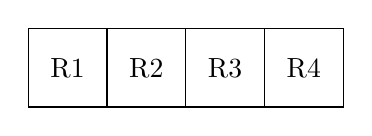
\begin{tikzpicture}
				\draw (0,0) rectangle (1,1) node[pos=.5] {R1};
				\draw (1,0) rectangle (2,1) node[pos=.5] {R2};
				\draw (2,0) rectangle (3,1) node[pos=.5] {R3};
				\draw (3,0) rectangle (4,1) node[pos=.5] {R4};
			\end{tikzpicture}
		\end{center}

		Die minimalen Rechtecke:
		\begin{center}
			\begin{tikzpicture}
				% border
				\draw (0,0) rectangle (6,6);

				\nodeA
				\nodeB
				\nodeC
				\nodeD

				\RA
				\RB
				\RC
				\RD
			\end{tikzpicture}
		\end{center}
	\end{solution}

	\item
	Fügen Sie anschließend die Einträge E, F und G in dieser Reihenfolge ein.


	\begin{solution}
		\paragraph{Einfügen von E}
		Das Einfügen von E führt zu einem Überlauf im Wurzelknoten, der gesplittet werden muss.
		Dazu müssen zwei neue Rechtecke über die bisherigen gelegt werden, die jeweils eine Teilmenge der vorhandenen Rechtecke überdecken.

		\begin{center}
			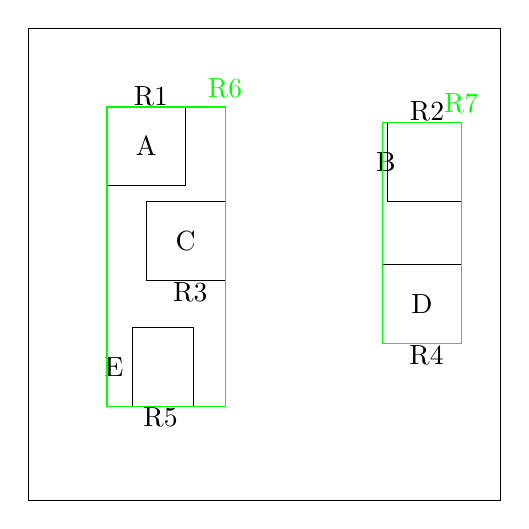
\begin{tikzpicture}
				% border
				\draw (0,0) rectangle (6,6);

				\nodeA
				\nodeB
				\nodeC
				\nodeD
				\nodeE

				\RA
				\RB
				\RC
				\RD

				\RE

				% root node
				\draw[color=green] (1  , 1.2) rectangle (2.5, 5  ) node[anchor=south] {R6};
				\draw[color=green] (4.5, 2.0) rectangle (5.5, 4.8) node[anchor=south] {R7};

			\end{tikzpicture}
		\end{center}

		Der Baum sieht dann so aus:
		\begin{center}
			\begin{tikzpicture}
				\draw (-1.5,0) rectangle (-0.5,1) node[name=R6,pos=.5] {R6};
				\draw (-0.5,0) rectangle (0.5,1) node[name=R7,pos=.5] {R7};
				\draw (0.5,0) rectangle (1.5,1) node[name=D1,pos=.5] {};
				\draw (1.5,0) rectangle (2.5,1) node[name=D2,pos=.5] {};

				\draw (-5,-2) rectangle (-4,-1) node[name=R1,pos=.5] {R1};
				\draw (-4,-2) rectangle (-3,-1) node[name=R3,pos=.5] {R3};
				\draw (-3,-2) rectangle (-2,-1) node[name=R5,pos=.5] {R5};
				\draw (-2,-2) rectangle (-1,-1) node[name=D3,pos=.5] {};

				\draw (1,-2) rectangle (2,-1) node[name=R2,pos=.5] {R2};
				\draw (2,-2) rectangle (3,-1) node[name=R4,pos=.5] {R4};
				\draw (3,-2) rectangle (4,-1) node[name=D4,pos=.5] {};
				\draw (4,-2) rectangle (5,-1) node[name=D5,pos=.5] {};

				\node[fit=(R1)(R3)(R5)(D3)](leftLeaf){};
				\node[fit=(R2)(R4)(D4)(D5)](rightLeaf){};

				\draw [thick, ->, >=stealth']
				([yshift=-2.5mm]R6.south) -- ([yshift=1mm]leftLeaf.north);
				\draw [thick, ->, >=stealth']
				([yshift=-2.5mm]R7.south) -- ([yshift=1mm]rightLeaf.north);
			\end{tikzpicture}
		\end{center}


		\paragraph{Wie wählt man diese neuen Rechtecke am sinnvollsten aus?}

		Ziel sollte sein, die Wahrscheinlichkeit zu minimieren, dass bei einem lesenden Zugriff beide Rechtecke und damit beide Teilbäume durchsucht werden müssen.

		Dies erreicht man z.\,B. dadurch, dass die Gesamtfläche beider Rechtecke minimal gewählt wird.
		Dazu schlägt Guttman verschiedene Strategien vor, die hier nicht weiter diskutiert werden sollen.

		\paragraph{Einfügen von F}

		Um F einzufügen, muss geklärt werden, welcher Blattknoten gewählt wird.
		Wird F bzw. sein minimales umgebendes Rechteck in einen Blattknoten eingefügt, so müssen alle umgebenden Rechtecke auf dem Weg von der Wurzel bis zum neuen Eintrag vergrößert werden.
		Dabei ist die Grundidee beim Absteigen des Baumes immer denjenigen Weg zu wählen, auf dem das jeweilige umgebende Rechteck am wenigsten vergrößert werden muss.

		Der Knoten F sollte also in den linken Blattknoten eingefügt werden, da das Rechteck R6 nur leicht vergrößert werden muss.
		Würde man ihn in den rechten Blattknoten einfügen, müsste das Rechteck R7 vergrößert werden, das dann mehr als vier mal größer wäre als ursprünglich.

		\begin{center}
			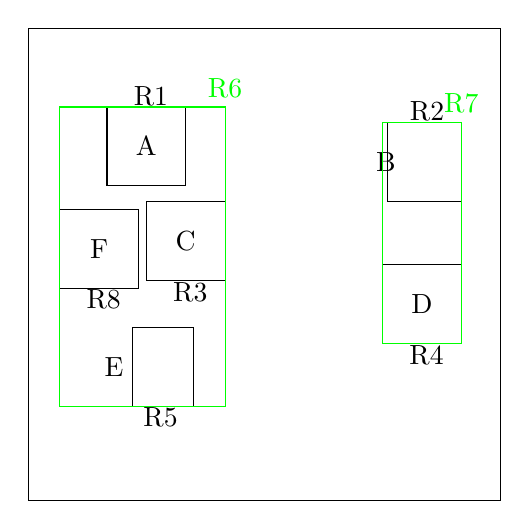
\begin{tikzpicture}
				% border
				\draw (0,0) rectangle (6,6);

				\nodeA
				\nodeB
				\nodeC
				\nodeD
				\nodeE
				\nodeF

				\RA
				\RB
				\RC
				\RD
				\RE
				\RF


				% root node
				\draw[color=green] (0.4  , 1.2) rectangle (2.5, 5  ) node[anchor=south] {R6};
				\draw[color=green] (4.5, 2.0) rectangle (5.5, 4.8) node[anchor=south] {R7};

			\end{tikzpicture}
		\end{center}


		\begin{center}
			\begin{tikzpicture}
				\draw (-1.5,0) rectangle (-0.5,1) node[name=R6,pos=.5] {R6};
				\draw (-0.5,0) rectangle (0.5,1) node[name=R7,pos=.5] {R7};
				\draw (0.5,0) rectangle (1.5,1) node[name=D1,pos=.5] {};
				\draw (1.5,0) rectangle (2.5,1) node[name=D2,pos=.5] {};

				\draw (-5,-2) rectangle (-4,-1) node[name=R1,pos=.5] {R1};
				\draw (-4,-2) rectangle (-3,-1) node[name=R3,pos=.5] {R3};
				\draw (-3,-2) rectangle (-2,-1) node[name=R5,pos=.5] {R5};
				\draw (-2,-2) rectangle (-1,-1) node[name=D3,pos=.5] {R8};

				\draw (1,-2) rectangle (2,-1) node[name=R2,pos=.5] {R2};
				\draw (2,-2) rectangle (3,-1) node[name=R4,pos=.5] {R4};
				\draw (3,-2) rectangle (4,-1) node[name=D4,pos=.5] {};
				\draw (4,-2) rectangle (5,-1) node[name=D5,pos=.5] {};

				\node[fit=(R1)(R3)(R5)(D3)](leftLeaf){};
				\node[fit=(R2)(R4)(D4)(D5)](rightLeaf){};

				\draw [thick, ->, >=stealth']
				([yshift=-2.5mm]R6.south) -- ([yshift=1mm]leftLeaf.north);
				\draw [thick, ->, >=stealth']
				([yshift=-2.5mm]R7.south) -- ([yshift=1mm]rightLeaf.north);
			\end{tikzpicture}
		\end{center}

		\paragraph{Einfügen von G}

		Soll G eingefügt werden, entsteht ein Überlauf im linken Blattknoten, der zum Splitt führt.
		Dazu wird R6 verkleinert und ein neues Rechteck R10 aufgespannt.
		Die in R6 ursprünglich enthaltenen Einträge werden so verteilt, dass R6 und R10 jeweils mindestens $m$ Einträge enthalten und die Gesamtfläche von R6 und R10 möglichst klein ist.

		\begin{center}
			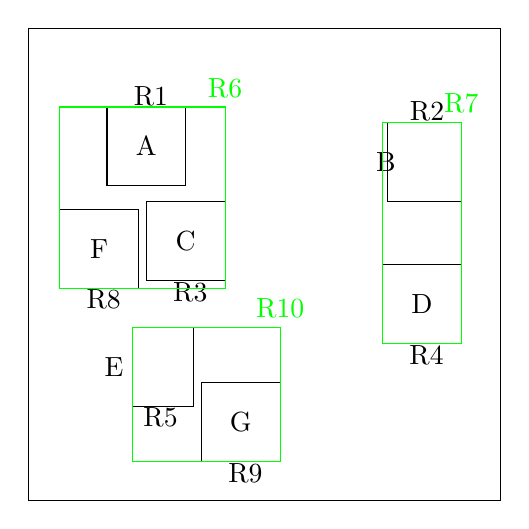
\begin{tikzpicture}
				% border
				\draw (0,0) rectangle (6,6);

				\nodeA
				\nodeB
				\nodeC
				\nodeD
				\nodeE
				\nodeF
				\nodeG

				\RA
				\RB
				\RC
				\RD
				\RE
				\RF
				\RG

				% root node
				\draw[color=green] (0.4, 2.7) rectangle (2.5, 5  ) node[anchor=south] {R6};
				\draw[color=green] (1.32, 0.5) rectangle (3.2, 2.2) node[anchor=south] {R10};
				\draw[color=green] (4.5, 2.0) rectangle (5.5, 4.8) node[anchor=south] {R7};

			\end{tikzpicture}
		\end{center}

		Der entstehende Baum sieht dann so aus:

		\begin{center}
			\begin{tikzpicture}
				\draw (0,0) rectangle (1,1) node[name=R6,pos=.5] {R6};
				\draw (1,0) rectangle (2,1) node[name=R10,pos=.5] {R10};
				\draw (2,0) rectangle (3,1) node[name=R7,pos=.5] {R7};
				\draw (3,0) rectangle (4,1) node[name=D2,pos=.5] {};

				\draw (-5,-2) rectangle (-4,-1) node[name=R1,pos=.5] {R1};
				\draw (-4,-2) rectangle (-3,-1) node[name=R3,pos=.5] {R3};
				\draw (-3,-2) rectangle (-2,-1) node[name=R8,pos=.5] {R8};
				\draw (-2,-2) rectangle (-1,-1) node[name=D3,pos=.5] {};

				\draw (0,-2) rectangle (1,-1) node[name=R5,pos=.5] {R5};
				\draw (1,-2) rectangle (2,-1) node[name=R9,pos=.5] {R9};
				\draw (2,-2) rectangle (3,-1) node[name=D4,pos=.5] {};
				\draw (3,-2) rectangle (4,-1) node[name=D5,pos=.5] {};

				\draw (5,-2) rectangle (6,-1) node[name=D6,pos=.5] {R2};
				\draw (6,-2) rectangle (7,-1) node[name=D7,pos=.5] {R4};
				\draw (7,-2) rectangle (8,-1) node[name=D8,pos=.5] {};
				\draw (8,-2) rectangle (9,-1) node[name=D9,pos=.5] {};

				\node[fit=(R1)(R3)(R8)(D3)](leftLeaf){};
				\node[fit=(R5)(R9)(D4)(D5)](centerLeaf){};
				\node[fit=(D6)(D7)(D8)(D9)](rightLeaf){};

				\draw [thick, ->, >=stealth']
				([yshift=-2.5mm]R6.south) -- ([yshift=1mm]leftLeaf.north);
				\draw [thick, ->, >=stealth']
				([yshift=-2.5mm]R10.south) -- ([yshift=1mm]centerLeaf.north);
				\draw [thick, ->, >=stealth']
				([yshift=-2.5mm]R7.south) -- ([yshift=1mm]rightLeaf.north);
			\end{tikzpicture}
		\end{center}

	\end{solution}
	\item Löschen Sie anschließend den Eintrag D.

	\begin{solution}
		Dies erzeugt einen Unterlauf im rechten Blattknoten.
		Nach Guttmans Algorithmus wird nun der gesamte Blattknoten und der Verweis auf ihn im Elternknoten gelöscht.
		Dadurch entsteht ein verwaister Eintrag (B in R2), dieser wird mit dem bereits bekannten Einfügealgorithmus erneut eingefügt.

		Dies ergibt folgendes Bild:

		\begin{center}
			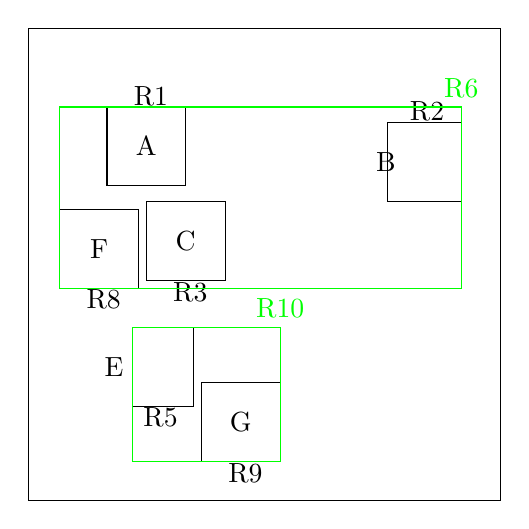
\begin{tikzpicture}
				% border
				\draw (0,0) rectangle (6,6);

				\nodeA
				\nodeB
				\nodeC
				\nodeE
				\nodeF
				\nodeG

				\RA
				\RB
				\RC
				\RE
				\RF
				\RG

				% root node
				\draw[color=green] (0.4, 2.7) rectangle (5.5, 5  ) node[anchor=south] {R6};
				\draw[color=green] (1.32, 0.5) rectangle (3.2, 2.2) node[anchor=south] {R10};

			\end{tikzpicture}
		\end{center}


		\begin{center}
			\begin{tikzpicture}
				\draw (0,0) rectangle (1,1) node[name=R6,pos=.5] {R6};
				\draw (1,0) rectangle (2,1) node[name=R10,pos=.5] {R10};
				\draw (2,0) rectangle (3,1) node[name=R7,pos=.5] {};
				\draw (3,0) rectangle (4,1) node[name=D2,pos=.5] {};

				\draw (-5,-2) rectangle (-4,-1) node[name=R1,pos=.5] {R1};
				\draw (-4,-2) rectangle (-3,-1) node[name=R3,pos=.5] {R3};
				\draw (-3,-2) rectangle (-2,-1) node[name=R8,pos=.5] {R8};
				\draw (-2,-2) rectangle (-1,-1) node[name=D3,pos=.5] {R2};

				\draw (1,-2) rectangle (2,-1) node[name=R5,pos=.5] {R5};
				\draw (2,-2) rectangle (3,-1) node[name=R9,pos=.5] {R9};
				\draw (3,-2) rectangle (4,-1) node[name=D4,pos=.5] {};
				\draw (4,-2) rectangle (5,-1) node[name=D5,pos=.5] {};

				\node[fit=(R1)(R3)(R8)(D3)](leftLeaf){};
				\node[fit=(R5)(R9)(D4)(D5)](centerLeaf){};
				\node[fit=(D6)(D7)(D8)(D9)](rightLeaf){};

				\draw [thick, ->, >=stealth']
				([yshift=-2.5mm]R6.south) -- ([yshift=1mm]leftLeaf.north);
				\draw [thick, ->, >=stealth']
				([yshift=-2.5mm]R10.south) -- ([yshift=1mm]centerLeaf.north);
			\end{tikzpicture}
		\end{center}



	\end{solution}


\end{enumerate}
